\newcommand{\NWtarget}[2]{#2}
\newcommand{\NWlink}[2]{#2}
\newcommand{\NWtxtMacroDefBy}{Fragment defined by}
\newcommand{\NWtxtMacroRefIn}{Fragment referenced in}
\newcommand{\NWtxtMacroNoRef}{Fragment never referenced}
\newcommand{\NWtxtDefBy}{Defined by}
\newcommand{\NWtxtRefIn}{Referenced in}
\newcommand{\NWtxtNoRef}{Not referenced}
\newcommand{\NWtxtFileDefBy}{File defined by}
\newcommand{\NWtxtIdentsUsed}{Uses:}
\newcommand{\NWtxtIdentsNotUsed}{Never used}
\newcommand{\NWtxtIdentsDefed}{Defines:}
\newcommand{\NWsep}{${\diamond}$}
\newcommand{\NWnotglobal}{(not defined globally)}
\newcommand{\NWuseHyperlinks}{}
\documentclass[12pt]{article}
\usepackage{graphicx}
\usepackage{amssymb}
\usepackage{listings}
\usepackage{amsmath}
\usepackage{graphicx}
\usepackage{float}
\usepackage[section]{placeins}
% Russian specicfic
% -------------------------
\usepackage[T2A]{fontenc}
\usepackage[utf8]{inputenc}
\usepackage[russian]{babel}
% -------------------------

\graphicspath{{./figs/}}

\begin{document}

\title{Общая связность сети. Критическое ребро.}

\author{
  Кирпа В. Д. (реализация, тестирование)
  \and
  Махлярчук Андрей (документация, тестирование)
  \and
  Утин Никита (визуализация, тестирование)
  \and
  Березкин Аркадий (реализация, документация)
}

\maketitle
\thispagestyle{empty}
\newpage

\tableofcontents
\listoffigures

\newpage

\section{Постановка задачи:}

\paragraph{}
Для графа $G = (V, E, W)$ с множеством вершин $V$,
множеством ребер $W: E \rightarrow \mathbb{R}_+$
найти ребро $e^*$, такое, что при замене
$W(e^*) \rightarrow \gamma W(e^*)$ сумма сетевых 
расстояний между всеми узлами минимизируется
(при $\gamma < 1$) или максимизируется (при $\gamma > 1$).

\section{Алгоритм}

\paragraph{}
Для нахождения суммы сетевых расстояний в графе использовался
алгоритм Дейкстры\cite{dijkstra}. Несмотря на то, что алгоритм
Дейкстры не подходит для несвязных графов, то, что он запускается
из каждой вершины позволяет его использовать, чтобы посчитать необходимую сумм.

\paragraph{}
Чтобы найти критическое ребро сумма сетевых расстояний считается
для всех графов $G_i$ таких, что $W(e_i) \rightarrow \gamma W(e_i)$. Если сетевые суммы 
в текущем графе $G_i$ меньше (больше при $\gamma > 1$)
ранее найденной суммы, то это ребро сохраняется в качестве претендента
на критическое. В конце работы алгоритма мы получаем критическое ребро, 
сумму сетевых расстояний, соответствующую графу с обновленным весом критического ребра и новый вес данного ребра.

\section{Реализация} 
В начале выполнения программы происходит считывание графа из файла. 
Во входном файле граф описывается в формате: $u v weight$, где $u$ и $v$ - номера вершин(тип $integer$), 
$weight$ - вес ребра (тип $double$).
Затем для каждой вершины запускаем алгоритм Дейкстры. В данной рализации можно было бы использовать 
алгоритм Флойда-Уоршелла, но было принято решение реализовать алгоритм Дейкстры, так как он легче поддается распараллеливанию.

\paragraph{}
Алгоритм реализован на языке C++. Основной процедурой является
алгоритм Дейкстры\cite{dijkstra}.

\subsection{Содержание исходного кода}


{\small\begin{list}{}{\setlength{\itemsep}{-\parsep}\setlength{\itemindent}{-\leftmargin}}
\item $\langle\,$constructors\nobreak\ {\footnotesize \NWlink{nuweb6a}{6a}}$\,\rangle$ {\footnotesize {\NWtxtRefIn} \NWlink{nuweb5}{5}.}
\item $\langle\,$getters and setters\nobreak\ {\footnotesize \NWlink{nuweb6b}{6b}}$\,\rangle$ {\footnotesize {\NWtxtRefIn} \NWlink{nuweb5}{5}.}
\item $\langle\,$gimpl add edge\nobreak\ {\footnotesize \NWlink{nuweb25a}{25a}}$\,\rangle$ {\footnotesize {\NWtxtRefIn} \NWlink{nuweb13b}{13b}.}
\item $\langle\,$gimpl constructors\nobreak\ {\footnotesize \NWlink{nuweb14a}{14a}}$\,\rangle$ {\footnotesize {\NWtxtRefIn} \NWlink{nuweb13b}{13b}.}
\item $\langle\,$gimpl critical init\nobreak\ {\footnotesize \NWlink{nuweb19b}{19b}}$\,\rangle$ {\footnotesize {\NWtxtRefIn} \NWlink{nuweb19a}{19a}.}
\item $\langle\,$gimpl critical max\nobreak\ {\footnotesize \NWlink{nuweb22}{22}}$\,\rangle$ {\footnotesize {\NWtxtRefIn} \NWlink{nuweb19a}{19a}.}
\item $\langle\,$gimpl critical min\nobreak\ {\footnotesize \NWlink{nuweb21}{21}}$\,\rangle$ {\footnotesize {\NWtxtRefIn} \NWlink{nuweb19a}{19a}.}
\item $\langle\,$gimpl critical print\nobreak\ {\footnotesize \NWlink{nuweb20}{20}}$\,\rangle$ {\footnotesize {\NWtxtRefIn} \NWlink{nuweb19a}{19a}.}
\item $\langle\,$gimpl critical search\nobreak\ {\footnotesize \NWlink{nuweb19a}{19a}}$\,\rangle$ {\footnotesize {\NWtxtRefIn} \NWlink{nuweb13b}{13b}.}
\item $\langle\,$gimpl dijkstra\nobreak\ {\footnotesize \NWlink{nuweb17a}{17a}}$\,\rangle$ {\footnotesize {\NWtxtRefIn} \NWlink{nuweb13b}{13b}.}
\item $\langle\,$gimpl Dijkstra algorythm\nobreak\ {\footnotesize \NWlink{nuweb23}{23}}$\,\rangle$ {\footnotesize {\NWtxtRefIn} \NWlink{nuweb13b}{13b}.}
\item $\langle\,$gimpl djk sum\nobreak\ {\footnotesize \NWlink{nuweb26}{26}}$\,\rangle$ {\footnotesize {\NWtxtRefIn} \NWlink{nuweb23}{23}.}
\item $\langle\,$gimpl djk vars\nobreak\ {\footnotesize \NWlink{nuweb24a}{24a}}$\,\rangle$ {\footnotesize {\NWtxtRefIn} \NWlink{nuweb23}{23}.}
\item $\langle\,$gimpl djk while\nobreak\ {\footnotesize \NWlink{nuweb25b}{25b}}$\,\rangle$ {\footnotesize {\NWtxtRefIn} \NWlink{nuweb23}{23}.}
\item $\langle\,$gimpl open\nobreak\ {\footnotesize \NWlink{nuweb14b}{14b}}$\,\rangle$ {\footnotesize {\NWtxtRefIn} \NWlink{nuweb13b}{13b}.}
\item $\langle\,$gimpl open for\nobreak\ {\footnotesize \NWlink{nuweb16b}{16b}}$\,\rangle$ {\footnotesize {\NWtxtRefIn} \NWlink{nuweb14b}{14b}.}
\item $\langle\,$gimpl open if\nobreak\ {\footnotesize \NWlink{nuweb16a}{16a}}$\,\rangle$ {\footnotesize {\NWtxtRefIn} \NWlink{nuweb15}{15}.}
\item $\langle\,$gimpl open while\nobreak\ {\footnotesize \NWlink{nuweb15}{15}}$\,\rangle$ {\footnotesize {\NWtxtRefIn} \NWlink{nuweb14b}{14b}.}
\item $\langle\,$gimpl run cycle\nobreak\ {\footnotesize \NWlink{nuweb18a}{18a}}$\,\rangle$ {\footnotesize {\NWtxtRefIn} \NWlink{nuweb17a}{17a}.}
\item $\langle\,$gimpl run Dijkstra\nobreak\ {\footnotesize \NWlink{nuweb24b}{24b}}$\,\rangle$ {\footnotesize {\NWtxtRefIn} \NWlink{nuweb13b}{13b}.}
\item $\langle\,$gimpl run sum\nobreak\ {\footnotesize \NWlink{nuweb18b}{18b}}$\,\rangle$ {\footnotesize {\NWtxtRefIn} \NWlink{nuweb17a}{17a}.}
\item $\langle\,$gimpl run threads\nobreak\ {\footnotesize \NWlink{nuweb17c}{17c}}$\,\rangle$ {\footnotesize {\NWtxtRefIn} \NWlink{nuweb17a}{17a}.}
\item $\langle\,$gimpl run threadscount\nobreak\ {\footnotesize \NWlink{nuweb17b}{17b}}$\,\rangle$ {\footnotesize {\NWtxtRefIn} \NWlink{nuweb17a}{17a}.}
\item $\langle\,$graph add edge\nobreak\ {\footnotesize \NWlink{nuweb12d}{12d}}$\,\rangle$ {\footnotesize {\NWtxtRefIn} \NWlink{nuweb8}{8}.}
\item $\langle\,$graph constructors\nobreak\ {\footnotesize \NWlink{nuweb9b}{9b}}$\,\rangle$ {\footnotesize {\NWtxtRefIn} \NWlink{nuweb8}{8}.}
\item $\langle\,$graph data\nobreak\ {\footnotesize \NWlink{nuweb11b}{11b}}$\,\rangle$ {\footnotesize {\NWtxtRefIn} \NWlink{nuweb8}{8}.}
\item $\langle\,$graph dijkstra\nobreak\ {\footnotesize \NWlink{nuweb10c}{10c}}$\,\rangle$ {\footnotesize {\NWtxtRefIn} \NWlink{nuweb8}{8}.}
\item $\langle\,$graph dijkstra2\nobreak\ {\footnotesize \NWlink{nuweb12b}{12b}}$\,\rangle$ {\footnotesize {\NWtxtRefIn} \NWlink{nuweb8}{8}.}
\item $\langle\,$graph distsum\nobreak\ {\footnotesize \NWlink{nuweb12a}{12a}}$\,\rangle$ {\footnotesize {\NWtxtRefIn} \NWlink{nuweb8}{8}.}
\item $\langle\,$graph edges\nobreak\ {\footnotesize \NWlink{nuweb10a}{10a}}$\,\rangle$ {\footnotesize {\NWtxtRefIn} \NWlink{nuweb8}{8}.}
\item $\langle\,$graph find critical\nobreak\ {\footnotesize \NWlink{nuweb10d}{10d}}$\,\rangle$ {\footnotesize {\NWtxtRefIn} \NWlink{nuweb8}{8}.}
\item $\langle\,$graph inf\nobreak\ {\footnotesize \NWlink{nuweb11a}{11a}}$\,\rangle$ {\footnotesize {\NWtxtRefIn} \NWlink{nuweb8}{8}.}
\item $\langle\,$graph open\nobreak\ {\footnotesize \NWlink{nuweb10b}{10b}}$\,\rangle$ {\footnotesize {\NWtxtRefIn} \NWlink{nuweb8}{8}.}
\item $\langle\,$graph operator\nobreak\ {\footnotesize \NWlink{nuweb13a}{13a}}$\,\rangle$ {\footnotesize {\NWtxtRefIn} \NWlink{nuweb8}{8}.}
\item $\langle\,$graph run dijkstra\nobreak\ {\footnotesize \NWlink{nuweb12c}{12c}}$\,\rangle$ {\footnotesize {\NWtxtRefIn} \NWlink{nuweb8}{8}.}
\item $\langle\,$graph used\nobreak\ {\footnotesize \NWlink{nuweb11c}{11c}}$\,\rangle$ {\footnotesize {\NWtxtRefIn} \NWlink{nuweb8}{8}.}
\item $\langle\,$includes\nobreak\ {\footnotesize \NWlink{nuweb9a}{9a}}$\,\rangle$ {\footnotesize {\NWtxtRefIn} \NWlink{nuweb8}{8}.}
\item $\langle\,$utilities\nobreak\ {\footnotesize \NWlink{nuweb7a}{7a}}$\,\rangle$ {\footnotesize {\NWtxtRefIn} \NWlink{nuweb5}{5}.}
\end{list}}

\subsection{Исходный код}
\paragraph{}
Ниже приведен код класса описывающего ребро графа.
\begin{flushleft} \small
\begin{minipage}{\linewidth}\label{scrap1}\raggedright\small
\NWtarget{nuweb5}{} \verb@"src/edge.h"@\nobreak\ {\footnotesize {5}}$\equiv$
\vspace{-1ex}
\begin{list}{}{} \item
\mbox{}\verb@@\\
\mbox{}\verb@#pragma once@\\
\mbox{}\verb@#include <atomic>@\\
\mbox{}\verb@#include <functional>@\\
\mbox{}\verb@@\\
\mbox{}\verb@class Edge {@\\
\mbox{}\verb@public:@\\
\mbox{}\verb@    @\hbox{$\langle\,${\itshape constructors}\nobreak\ {\footnotesize \NWlink{nuweb6a}{6a}}$\,\rangle$}\verb@@\\
\mbox{}\verb@    @\hbox{$\langle\,${\itshape getters and setters}\nobreak\ {\footnotesize \NWlink{nuweb6b}{6b}}$\,\rangle$}\verb@@\\
\mbox{}\verb@private:@\\
\mbox{}\verb@    int left;@\\
\mbox{}\verb@    int right;@\\
\mbox{}\verb@    double weight;@\\
\mbox{}\verb@    int id;@\\
\mbox{}\verb@};@\\
\mbox{}\verb@@\\
\mbox{}\verb@@\hbox{$\langle\,${\itshape utilities}\nobreak\ {\footnotesize \NWlink{nuweb7a}{7a}}$\,\rangle$}\verb@@\\
\mbox{}\verb@@\\
\mbox{}\verb@@{\NWsep}
\end{list}
\vspace{-1.5ex}
\footnotesize
\begin{list}{}{\setlength{\itemsep}{-\parsep}\setlength{\itemindent}{-\leftmargin}}

\item{}
\end{list}
\end{minipage}\vspace{4ex}
\end{flushleft}
\paragraph{}
Класс имеет 2 конструктора, один из которых конструктор копирования.
Конструктор принимает 2 номера соединяемых вершин типа $int$, 
вес ребра типа $double$ и уникальный $id$ типа $int$, для того чтобы 
можно было эффективно искать ребра. Эти данные сохраняются в качестве
полей объекта. 

\begin{flushleft} \small
\begin{minipage}{\linewidth}\label{scrap2}\raggedright\small
\NWtarget{nuweb6a}{} $\langle\,${\itshape constructors}\nobreak\ {\footnotesize {6a}}$\,\rangle\equiv$
\vspace{-1ex}
\begin{list}{}{} \item
\mbox{}\verb@@\\
\mbox{}\verb@Edge(const Edge& e) :@\\
\mbox{}\verb@    left(e.left), @\\
\mbox{}\verb@    right(e.right), @\\
\mbox{}\verb@    weight(e.weight), @\\
\mbox{}\verb@    id(e.id) { }@\\
\mbox{}\verb@Edge(int u, int v, double w, int id) : @\\
\mbox{}\verb@    left(u), @\\
\mbox{}\verb@    right(v), @\\
\mbox{}\verb@    weight(w), @\\
\mbox{}\verb@    id(id) { }@\\
\mbox{}\verb@@{\NWsep}
\end{list}
\vspace{-1.5ex}
\footnotesize
\begin{list}{}{\setlength{\itemsep}{-\parsep}\setlength{\itemindent}{-\leftmargin}}
\item \NWtxtMacroRefIn\ \NWlink{nuweb5}{5}.

\item{}
\end{list}
\end{minipage}\vspace{4ex}
\end{flushleft}
\paragraph{}
Класс имеет геттеры для всех полей объектов и сеттер для поля $weight$, т.к.
необходимо динамически изменять вес ребер в графе, чтобы пересчитывать суммы сетевых расстояний.

\begin{flushleft} \small
\begin{minipage}{\linewidth}\label{scrap3}\raggedright\small
\NWtarget{nuweb6b}{} $\langle\,${\itshape getters and setters}\nobreak\ {\footnotesize {6b}}$\,\rangle\equiv$
\vspace{-1ex}
\begin{list}{}{} \item
\mbox{}\verb@@\\
\mbox{}\verb@const int GetLeft() const { return left; }@\\
\mbox{}\verb@const int GetRight() const { return right; }@\\
\mbox{}\verb@const double GetWeight() const { return weight; }@\\
\mbox{}\verb@const int getId() const { return id; }@\\
\mbox{}\verb@void SetWeight(double w) { weight = w; }@\\
\mbox{}\verb@@{\NWsep}
\end{list}
\vspace{-1.5ex}
\footnotesize
\begin{list}{}{\setlength{\itemsep}{-\parsep}\setlength{\itemindent}{-\leftmargin}}
\item \NWtxtMacroRefIn\ \NWlink{nuweb5}{5}.

\item{}
\end{list}
\end{minipage}\vspace{4ex}
\end{flushleft}
\paragraph{}
Для удобства использования структутры были написаны оператор "()" 
обеспечивающий возможность удобного доступа к элементам и оператор сравнения.

\begin{flushleft} \small
\begin{minipage}{\linewidth}\label{scrap4}\raggedright\small
\NWtarget{nuweb7a}{} $\langle\,${\itshape utilities}\nobreak\ {\footnotesize {7a}}$\,\rangle\equiv$
\vspace{-1ex}
\begin{list}{}{} \item
\mbox{}\verb@@\\
\mbox{}\verb@struct EdgeHash {@\\
\mbox{}\verb@    unsigned int operator()(const Edge& e) const {@\\
\mbox{}\verb@        return std::hash<int>()(e.GetRight());@\\
\mbox{}\verb@    }@\\
\mbox{}\verb@};@\\
\mbox{}\verb@@\\
\mbox{}\verb@bool operator==(const Edge& e, const Edge& t);@\\
\mbox{}\verb@@{\NWsep}
\end{list}
\vspace{-1.5ex}
\footnotesize
\begin{list}{}{\setlength{\itemsep}{-\parsep}\setlength{\itemindent}{-\leftmargin}}
\item \NWtxtMacroRefIn\ \NWlink{nuweb5}{5}.

\item{}
\end{list}
\end{minipage}\vspace{4ex}
\end{flushleft}
\begin{flushleft} \small
\begin{minipage}{\linewidth}\label{scrap5}\raggedright\small
\NWtarget{nuweb7b}{} \verb@"src/edge.cpp"@\nobreak\ {\footnotesize {7b}}$\equiv$
\vspace{-1ex}
\begin{list}{}{} \item
\mbox{}\verb@@\\
\mbox{}\verb@#include "edge.h"@\\
\mbox{}\verb@@\\
\mbox{}\verb@bool operator==(const Edge& e, const Edge& t) {@\\
\mbox{}\verb@    return e.GetRight() == t.GetRight();@\\
\mbox{}\verb@}@\\
\mbox{}\verb@@{\NWsep}
\end{list}
\vspace{-1.5ex}
\footnotesize
\begin{list}{}{\setlength{\itemsep}{-\parsep}\setlength{\itemindent}{-\leftmargin}}

\item{}
\end{list}
\end{minipage}\vspace{4ex}
\end{flushleft}
\paragraph{}
Код класса описывающий граф.

\begin{flushleft} \small
\begin{minipage}{\linewidth}\label{scrap6}\raggedright\small
\NWtarget{nuweb8}{} \verb@"src/graph.h"@\nobreak\ {\footnotesize {8}}$\equiv$
\vspace{-1ex}
\begin{list}{}{} \item
\mbox{}\verb@@\\
\mbox{}\verb@@\hbox{$\langle\,${\itshape includes}\nobreak\ {\footnotesize \NWlink{nuweb9a}{9a}}$\,\rangle$}\verb@@\\
\mbox{}\verb@class Graph {@\\
\mbox{}\verb@public:@\\
\mbox{}\verb@    @\hbox{$\langle\,${\itshape graph constructors}\nobreak\ {\footnotesize \NWlink{nuweb9b}{9b}}$\,\rangle$}\verb@@\\
\mbox{}\verb@    @\hbox{$\langle\,${\itshape graph edges}\nobreak\ {\footnotesize \NWlink{nuweb10a}{10a}}$\,\rangle$}\verb@@\\
\mbox{}\verb@    @\hbox{$\langle\,${\itshape graph open}\nobreak\ {\footnotesize \NWlink{nuweb10b}{10b}}$\,\rangle$}\verb@@\\
\mbox{}\verb@    @\hbox{$\langle\,${\itshape graph dijkstra}\nobreak\ {\footnotesize \NWlink{nuweb10c}{10c}}$\,\rangle$}\verb@@\\
\mbox{}\verb@    @\hbox{$\langle\,${\itshape graph find critical}\nobreak\ {\footnotesize \NWlink{nuweb10d}{10d}}$\,\rangle$}\verb@@\\
\mbox{}\verb@private:@\\
\mbox{}\verb@    @\hbox{$\langle\,${\itshape graph inf}\nobreak\ {\footnotesize \NWlink{nuweb11a}{11a}}$\,\rangle$}\verb@@\\
\mbox{}\verb@    @\hbox{$\langle\,${\itshape graph data}\nobreak\ {\footnotesize \NWlink{nuweb11b}{11b}}$\,\rangle$}\verb@@\\
\mbox{}\verb@    @\hbox{$\langle\,${\itshape graph used}\nobreak\ {\footnotesize \NWlink{nuweb11c}{11c}}$\,\rangle$}\verb@@\\
\mbox{}\verb@    @\hbox{$\langle\,${\itshape graph distsum}\nobreak\ {\footnotesize \NWlink{nuweb12a}{12a}}$\,\rangle$}\verb@@\\
\mbox{}\verb@    @\hbox{$\langle\,${\itshape graph dijkstra2}\nobreak\ {\footnotesize \NWlink{nuweb12b}{12b}}$\,\rangle$}\verb@@\\
\mbox{}\verb@    @\hbox{$\langle\,${\itshape graph run dijkstra}\nobreak\ {\footnotesize \NWlink{nuweb12c}{12c}}$\,\rangle$}\verb@@\\
\mbox{}\verb@    @\hbox{$\langle\,${\itshape graph add edge}\nobreak\ {\footnotesize \NWlink{nuweb12d}{12d}}$\,\rangle$}\verb@@\\
\mbox{}\verb@};@\\
\mbox{}\verb@@\\
\mbox{}\verb@    @\hbox{$\langle\,${\itshape graph operator}\nobreak\ {\footnotesize \NWlink{nuweb13a}{13a}}$\,\rangle$}\verb@@\\
\mbox{}\verb@@{\NWsep}
\end{list}
\vspace{-1.5ex}
\footnotesize
\begin{list}{}{\setlength{\itemsep}{-\parsep}\setlength{\itemindent}{-\leftmargin}}

\item{}
\end{list}
\end{minipage}\vspace{4ex}
\end{flushleft}
\paragraph{}
Зависимости класса описывающего граф.

\begin{flushleft} \small
\begin{minipage}{\linewidth}\label{scrap7}\raggedright\small
\NWtarget{nuweb9a}{} $\langle\,${\itshape includes}\nobreak\ {\footnotesize {9a}}$\,\rangle\equiv$
\vspace{-1ex}
\begin{list}{}{} \item
\mbox{}\verb@@\\
\mbox{}\verb@#pragma once@\\
\mbox{}\verb@#include <unordered_map>@\\
\mbox{}\verb@#include <unordered_set>@\\
\mbox{}\verb@#include <set>@\\
\mbox{}\verb@#include <iostream>@\\
\mbox{}\verb@#include <fstream>@\\
\mbox{}\verb@#include <queue>@\\
\mbox{}\verb@#include <string>@\\
\mbox{}\verb@#include <atomic>@\\
\mbox{}\verb@#include <thread>@\\
\mbox{}\verb@#include <sstream>@\\
\mbox{}\verb@#include <regex>@\\
\mbox{}\verb@#include "edge.h"@\\
\mbox{}\verb@#include <cfloat>@\\
\mbox{}\verb@@{\NWsep}
\end{list}
\vspace{-1.5ex}
\footnotesize
\begin{list}{}{\setlength{\itemsep}{-\parsep}\setlength{\itemindent}{-\leftmargin}}
\item \NWtxtMacroRefIn\ \NWlink{nuweb8}{8}.

\item{}
\end{list}
\end{minipage}\vspace{4ex}
\end{flushleft}
\paragraph{}
Конструкторы класса описывающего граф.

\begin{flushleft} \small
\begin{minipage}{\linewidth}\label{scrap8}\raggedright\small
\NWtarget{nuweb9b}{} $\langle\,${\itshape graph constructors}\nobreak\ {\footnotesize {9b}}$\,\rangle\equiv$
\vspace{-1ex}
\begin{list}{}{} \item
\mbox{}\verb@@\\
\mbox{}\verb@Graph();@\\
\mbox{}\verb@Graph(std::string filename);@\\
\mbox{}\verb@@{\NWsep}
\end{list}
\vspace{-1.5ex}
\footnotesize
\begin{list}{}{\setlength{\itemsep}{-\parsep}\setlength{\itemindent}{-\leftmargin}}
\item \NWtxtMacroRefIn\ \NWlink{nuweb8}{8}.

\item{}
\end{list}
\end{minipage}\vspace{4ex}
\end{flushleft}
\paragraph{}
Поле для хранения ребер графа. Для эффективности вычислений используется std::unordered\_map. 

\begin{flushleft} \small
\begin{minipage}{\linewidth}\label{scrap9}\raggedright\small
\NWtarget{nuweb10a}{} $\langle\,${\itshape graph edges}\nobreak\ {\footnotesize {10a}}$\,\rangle\equiv$
\vspace{-1ex}
\begin{list}{}{} \item
\mbox{}\verb@@\\
\mbox{}\verb@std::unordered_map <int, std::unordered_set <Edge, EdgeHash>> edges;@\\
\mbox{}\verb@@{\NWsep}
\end{list}
\vspace{-1.5ex}
\footnotesize
\begin{list}{}{\setlength{\itemsep}{-\parsep}\setlength{\itemindent}{-\leftmargin}}
\item \NWtxtMacroRefIn\ \NWlink{nuweb8}{8}.

\item{}
\end{list}
\end{minipage}\vspace{4ex}
\end{flushleft}
\paragraph{}
Функция для считывания графа из файла.

\begin{flushleft} \small
\begin{minipage}{\linewidth}\label{scrap10}\raggedright\small
\NWtarget{nuweb10b}{} $\langle\,${\itshape graph open}\nobreak\ {\footnotesize {10b}}$\,\rangle\equiv$
\vspace{-1ex}
\begin{list}{}{} \item
\mbox{}\verb@@\\
\mbox{}\verb@void open(std::string filename);@\\
\mbox{}\verb@@{\NWsep}
\end{list}
\vspace{-1.5ex}
\footnotesize
\begin{list}{}{\setlength{\itemsep}{-\parsep}\setlength{\itemindent}{-\leftmargin}}
\item \NWtxtMacroRefIn\ \NWlink{nuweb8}{8}.

\item{}
\end{list}
\end{minipage}\vspace{4ex}
\end{flushleft}
\paragraph{}
Функция,запускающая алгоритм Дейкстры в разных потоках.
\begin{flushleft} \small
\begin{minipage}{\linewidth}\label{scrap11}\raggedright\small
\NWtarget{nuweb10c}{} $\langle\,${\itshape graph dijkstra}\nobreak\ {\footnotesize {10c}}$\,\rangle\equiv$
\vspace{-1ex}
\begin{list}{}{} \item
\mbox{}\verb@@\\
\mbox{}\verb@double RunDijkstraAsync();    @\\
\mbox{}\verb@@{\NWsep}
\end{list}
\vspace{-1.5ex}
\footnotesize
\begin{list}{}{\setlength{\itemsep}{-\parsep}\setlength{\itemindent}{-\leftmargin}}
\item \NWtxtMacroRefIn\ \NWlink{nuweb8}{8}.

\item{}
\end{list}
\end{minipage}\vspace{4ex}
\end{flushleft}
\paragraph{}
Основная функция, осуществляющая поиск критического ребра в исходном графе. В качестве аргумента принимает значение $\gamma$
из исходной задачи.
\begin{flushleft} \small
\begin{minipage}{\linewidth}\label{scrap12}\raggedright\small
\NWtarget{nuweb10d}{} $\langle\,${\itshape graph find critical}\nobreak\ {\footnotesize {10d}}$\,\rangle\equiv$
\vspace{-1ex}
\begin{list}{}{} \item
\mbox{}\verb@@\\
\mbox{}\verb@void FindCriticalEdge(double k);@\\
\mbox{}\verb@@{\NWsep}
\end{list}
\vspace{-1.5ex}
\footnotesize
\begin{list}{}{\setlength{\itemsep}{-\parsep}\setlength{\itemindent}{-\leftmargin}}
\item \NWtxtMacroRefIn\ \NWlink{nuweb8}{8}.

\item{}
\end{list}
\end{minipage}\vspace{4ex}
\end{flushleft}
\paragraph{}
Константа имтирующая бесконечность в поиске путей алгоритмом Дейкстры.
\begin{flushleft} \small
\begin{minipage}{\linewidth}\label{scrap13}\raggedright\small
\NWtarget{nuweb11a}{} $\langle\,${\itshape graph inf}\nobreak\ {\footnotesize {11a}}$\,\rangle\equiv$
\vspace{-1ex}
\begin{list}{}{} \item
\mbox{}\verb@@\\
\mbox{}\verb@static const long long inf = std::numeric_limits<long long>::max();@\\
\mbox{}\verb@@{\NWsep}
\end{list}
\vspace{-1.5ex}
\footnotesize
\begin{list}{}{\setlength{\itemsep}{-\parsep}\setlength{\itemindent}{-\leftmargin}}
\item \NWtxtMacroRefIn\ \NWlink{nuweb8}{8}.

\item{}
\end{list}
\end{minipage}\vspace{4ex}
\end{flushleft}
\paragraph{}
Поля необходимые для хранения перенумерованных вершин графа.

\begin{flushleft} \small
\begin{minipage}{\linewidth}\label{scrap14}\raggedright\small
\NWtarget{nuweb11b}{} $\langle\,${\itshape graph data}\nobreak\ {\footnotesize {11b}}$\,\rangle\equiv$
\vspace{-1ex}
\begin{list}{}{} \item
\mbox{}\verb@@\\
\mbox{}\verb@std::unordered_map<int, int> coord;@\\
\mbox{}\verb@std::unordered_map<int, int> coord_to_vertecies;@\\
\mbox{}\verb@@{\NWsep}
\end{list}
\vspace{-1.5ex}
\footnotesize
\begin{list}{}{\setlength{\itemsep}{-\parsep}\setlength{\itemindent}{-\leftmargin}}
\item \NWtxtMacroRefIn\ \NWlink{nuweb8}{8}.

\item{}
\end{list}
\end{minipage}\vspace{4ex}
\end{flushleft}
\paragraph{}
Структура данных, сохраняющая индексы использованных ребер. 
\begin{flushleft} \small
\begin{minipage}{\linewidth}\label{scrap15}\raggedright\small
\NWtarget{nuweb11c}{} $\langle\,${\itshape graph used}\nobreak\ {\footnotesize {11c}}$\,\rangle\equiv$
\vspace{-1ex}
\begin{list}{}{} \item
\mbox{}\verb@@\\
\mbox{}\verb@std::unordered_set<int> usedEdges;@\\
\mbox{}\verb@@{\NWsep}
\end{list}
\vspace{-1.5ex}
\footnotesize
\begin{list}{}{\setlength{\itemsep}{-\parsep}\setlength{\itemindent}{-\leftmargin}}
\item \NWtxtMacroRefIn\ \NWlink{nuweb8}{8}.

\item{}
\end{list}
\end{minipage}\vspace{4ex}
\end{flushleft}
\paragraph{}
Массив необходимый для хранения сетевых расстояний, получаемых алгоритмом Дейкстры, запущенным в разных потоках. 
\begin{flushleft} \small
\begin{minipage}{\linewidth}\label{scrap16}\raggedright\small
\NWtarget{nuweb12a}{} $\langle\,${\itshape graph distsum}\nobreak\ {\footnotesize {12a}}$\,\rangle\equiv$
\vspace{-1ex}
\begin{list}{}{} \item
\mbox{}\verb@@\\
\mbox{}\verb@std::vector<double> distSum;@\\
\mbox{}\verb@@{\NWsep}
\end{list}
\vspace{-1.5ex}
\footnotesize
\begin{list}{}{\setlength{\itemsep}{-\parsep}\setlength{\itemindent}{-\leftmargin}}
\item \NWtxtMacroRefIn\ \NWlink{nuweb8}{8}.

\item{}
\end{list}
\end{minipage}\vspace{4ex}
\end{flushleft}
\paragraph{}
Функция реализующая алгоритм Дейкстры. Принимает на вход номер вершины.
\begin{flushleft} \small
\begin{minipage}{\linewidth}\label{scrap17}\raggedright\small
\NWtarget{nuweb12b}{} $\langle\,${\itshape graph dijkstra2}\nobreak\ {\footnotesize {12b}}$\,\rangle\equiv$
\vspace{-1ex}
\begin{list}{}{} \item
\mbox{}\verb@@\\
\mbox{}\verb@double Dijkstra(int v);@\\
\mbox{}\verb@@{\NWsep}
\end{list}
\vspace{-1.5ex}
\footnotesize
\begin{list}{}{\setlength{\itemsep}{-\parsep}\setlength{\itemindent}{-\leftmargin}}
\item \NWtxtMacroRefIn\ \NWlink{nuweb8}{8}.

\item{}
\end{list}
\end{minipage}\vspace{4ex}
\end{flushleft}
\paragraph{}
Функция запускающая алгоритм дейкстры $Dijkstra(int v)$.
\begin{flushleft} \small
\begin{minipage}{\linewidth}\label{scrap18}\raggedright\small
\NWtarget{nuweb12c}{} $\langle\,${\itshape graph run dijkstra}\nobreak\ {\footnotesize {12c}}$\,\rangle\equiv$
\vspace{-1ex}
\begin{list}{}{} \item
\mbox{}\verb@@\\
\mbox{}\verb@void RunDijkstraThread(int from, int len);@\\
\mbox{}\verb@@{\NWsep}
\end{list}
\vspace{-1.5ex}
\footnotesize
\begin{list}{}{\setlength{\itemsep}{-\parsep}\setlength{\itemindent}{-\leftmargin}}
\item \NWtxtMacroRefIn\ \NWlink{nuweb8}{8}.

\item{}
\end{list}
\end{minipage}\vspace{4ex}
\end{flushleft}
\paragraph{}
Функция, добавляющая ребро в граф. Принимает на вход номера вершин (u, v), вес, индекс нового ребра.
\begin{flushleft} \small
\begin{minipage}{\linewidth}\label{scrap19}\raggedright\small
\NWtarget{nuweb12d}{} $\langle\,${\itshape graph add edge}\nobreak\ {\footnotesize {12d}}$\,\rangle\equiv$
\vspace{-1ex}
\begin{list}{}{} \item
\mbox{}\verb@@\\
\mbox{}\verb@void AddEdge(int u, int v, double weight, int id);   @\\
\mbox{}\verb@@{\NWsep}
\end{list}
\vspace{-1.5ex}
\footnotesize
\begin{list}{}{\setlength{\itemsep}{-\parsep}\setlength{\itemindent}{-\leftmargin}}
\item \NWtxtMacroRefIn\ \NWlink{nuweb8}{8}.

\item{}
\end{list}
\end{minipage}\vspace{4ex}
\end{flushleft}
\paragraph{}
Для удобства сравнения объектов класса перегружен слудющий оператор.
\begin{flushleft} \small
\begin{minipage}{\linewidth}\label{scrap20}\raggedright\small
\NWtarget{nuweb13a}{} $\langle\,${\itshape graph operator}\nobreak\ {\footnotesize {13a}}$\,\rangle\equiv$
\vspace{-1ex}
\begin{list}{}{} \item
\mbox{}\verb@@\\
\mbox{}\verb@class Compare {@\\
\mbox{}\verb@public:@\\
\mbox{}\verb@    bool operator()(std::pair<double, int> a, std::pair<double, int> b) {@\\
\mbox{}\verb@        return a.first > b.first;@\\
\mbox{}\verb@    }@\\
\mbox{}\verb@};@\\
\mbox{}\verb@@{\NWsep}
\end{list}
\vspace{-1.5ex}
\footnotesize
\begin{list}{}{\setlength{\itemsep}{-\parsep}\setlength{\itemindent}{-\leftmargin}}
\item \NWtxtMacroRefIn\ \NWlink{nuweb8}{8}.

\item{}
\end{list}
\end{minipage}\vspace{4ex}
\end{flushleft}
Ниже приведена реализация функций описанного выше класса в $graph.h$

\begin{flushleft} \small\label{scrap21}\raggedright\small
\NWtarget{nuweb13b}{} \verb@"src/graph.cpp"@\nobreak\ {\footnotesize {13b}}$\equiv$
\vspace{-1ex}
\begin{list}{}{} \item
\mbox{}\verb@@\\
\mbox{}\verb@#include <vector>@\\
\mbox{}\verb@#include "graph.h"@\\
\mbox{}\verb@@\\
\mbox{}\verb@using namespace std;@\\
\mbox{}\verb@@\\
\mbox{}\verb@//Public methods@\\
\mbox{}\verb@@\hbox{$\langle\,${\itshape gimpl constructors}\nobreak\ {\footnotesize \NWlink{nuweb14a}{14a}}$\,\rangle$}\verb@@\\
\mbox{}\verb@@\hbox{$\langle\,${\itshape gimpl open}\nobreak\ {\footnotesize \NWlink{nuweb14b}{14b}}$\,\rangle$}\verb@@\\
\mbox{}\verb@@\hbox{$\langle\,${\itshape gimpl dijkstra}\nobreak\ {\footnotesize \NWlink{nuweb17a}{17a}}$\,\rangle$}\verb@@\\
\mbox{}\verb@@\hbox{$\langle\,${\itshape gimpl critical search}\nobreak\ {\footnotesize \NWlink{nuweb19a}{19a}}$\,\rangle$}\verb@@\\
\mbox{}\verb@@\hbox{$\langle\,${\itshape gimpl Dijkstra algorythm}\nobreak\ {\footnotesize \NWlink{nuweb23}{23}}$\,\rangle$}\verb@@\\
\mbox{}\verb@@\hbox{$\langle\,${\itshape gimpl run Dijkstra}\nobreak\ {\footnotesize \NWlink{nuweb24b}{24b}}$\,\rangle$}\verb@@\\
\mbox{}\verb@@\hbox{$\langle\,${\itshape gimpl add edge}\nobreak\ {\footnotesize \NWlink{nuweb25a}{25a}}$\,\rangle$}\verb@@\\
\mbox{}\verb@@{\NWsep}
\end{list}
\vspace{-1.5ex}
\footnotesize
\begin{list}{}{\setlength{\itemsep}{-\parsep}\setlength{\itemindent}{-\leftmargin}}

\item{}
\end{list}
\vspace{4ex}
\end{flushleft}
\paragraph{}
Имплементация конструкторов графа. Перегруженный конструктор принимает на вход имя файла, содержащего
данные об исходном графе.

\begin{flushleft} \small
\begin{minipage}{\linewidth}\label{scrap22}\raggedright\small
\NWtarget{nuweb14a}{} $\langle\,${\itshape gimpl constructors}\nobreak\ {\footnotesize {14a}}$\,\rangle\equiv$
\vspace{-1ex}
\begin{list}{}{} \item
\mbox{}\verb@@\\
\mbox{}\verb@Graph::Graph() { }@\\
\mbox{}\verb@@\\
\mbox{}\verb@Graph::Graph(std::string filename) {@\\
\mbox{}\verb@    open(filename);@\\
\mbox{}\verb@} @\\
\mbox{}\verb@@{\NWsep}
\end{list}
\vspace{-1.5ex}
\footnotesize
\begin{list}{}{\setlength{\itemsep}{-\parsep}\setlength{\itemindent}{-\leftmargin}}
\item \NWtxtMacroRefIn\ \NWlink{nuweb13b}{13b}.

\item{}
\end{list}
\end{minipage}\vspace{4ex}
\end{flushleft}
\paragraph{}
Функция считывания файла с исходным графом.

\begin{flushleft} \small
\begin{minipage}{\linewidth}\label{scrap23}\raggedright\small
\NWtarget{nuweb14b}{} $\langle\,${\itshape gimpl open}\nobreak\ {\footnotesize {14b}}$\,\rangle\equiv$
\vspace{-1ex}
\begin{list}{}{} \item
\mbox{}\verb@@\\
\mbox{}\verb@void Graph::open(std::string filename) {@\\
\mbox{}\verb@    if (filename != "") {@\\
\mbox{}\verb@        std::ifstream in(filename);@\\
\mbox{}\verb@        int index, vertex;@\\
\mbox{}\verb@        double weight;@\\
\mbox{}\verb@        int n = 0;@\\
\mbox{}\verb@        int id = 0;@\\
\mbox{}\verb@        @\hbox{$\langle\,${\itshape gimpl open while}\nobreak\ {\footnotesize \NWlink{nuweb15}{15}}$\,\rangle$}\verb@@\\
\mbox{}\verb@@\\
\mbox{}\verb@        @\hbox{$\langle\,${\itshape gimpl open for}\nobreak\ {\footnotesize \NWlink{nuweb16b}{16b}}$\,\rangle$}\verb@@\\
\mbox{}\verb@    }@\\
\mbox{}\verb@    distSum.resize(edges.size(), 0);@\\
\mbox{}\verb@} @\\
\mbox{}\verb@@{\NWsep}
\end{list}
\vspace{-1.5ex}
\footnotesize
\begin{list}{}{\setlength{\itemsep}{-\parsep}\setlength{\itemindent}{-\leftmargin}}
\item \NWtxtMacroRefIn\ \NWlink{nuweb13b}{13b}.

\item{}
\end{list}
\end{minipage}\vspace{4ex}
\end{flushleft}
\paragraph{}
Цикл, предназначенный для считывния ребер графа и перенумировывания вершин графа, 
с целью иметь возможность заменить в основной структуре, содержащей граф std::unordered\_map на std::vector
и не столкнуться с ограничениями, связанными с размером памяти. Заменить std::unordered\_map на std::vector может
потребоваться в случае, если мы хотим добиться большей производительности, так как стандартный шаблонный класс
std::vector более оптимизирован для работы с различными уровнями кэша процессора.

\begin{flushleft} \small
\begin{minipage}{\linewidth}\label{scrap24}\raggedright\small
\NWtarget{nuweb15}{} $\langle\,${\itshape gimpl open while}\nobreak\ {\footnotesize {15}}$\,\rangle\equiv$
\vspace{-1ex}
\begin{list}{}{} \item
\mbox{}\verb@@\\
\mbox{}\verb@while (!in.eof()) {@\\
\mbox{}\verb@          int v;@\\
\mbox{}\verb@          int u;@\\
\mbox{}\verb@          in >> index >> vertex >> weight;@\\
\mbox{}\verb@@\\
\mbox{}\verb@          @\hbox{$\langle\,${\itshape gimpl open if}\nobreak\ {\footnotesize \NWlink{nuweb16a}{16a}}$\,\rangle$}\verb@@\\
\mbox{}\verb@@\\
\mbox{}\verb@          @\\
\mbox{}\verb@          AddEdge(u, v, weight, id++);@\\
\mbox{}\verb@          AddEdge(v, u, weight, id++);@\\
\mbox{}\verb@} @\\
\mbox{}\verb@@{\NWsep}
\end{list}
\vspace{-1.5ex}
\footnotesize
\begin{list}{}{\setlength{\itemsep}{-\parsep}\setlength{\itemindent}{-\leftmargin}}
\item \NWtxtMacroRefIn\ \NWlink{nuweb14b}{14b}.

\item{}
\end{list}
\end{minipage}\vspace{4ex}
\end{flushleft}
\paragraph{}
Проверка на то, не встречалась ли нам эта вершина ранее в процессе считывания исходного графа.
\begin{flushleft} \small
\begin{minipage}{\linewidth}\label{scrap25}\raggedright\small
\NWtarget{nuweb16a}{} $\langle\,${\itshape gimpl open if}\nobreak\ {\footnotesize {16a}}$\,\rangle\equiv$
\vspace{-1ex}
\begin{list}{}{} \item
\mbox{}\verb@@\\
\mbox{}\verb@if (coord.find(index) != coord.end()) {@\\
\mbox{}\verb@    v = coord[index];@\\
\mbox{}\verb@} @\\
\mbox{}\verb@else {@\\
\mbox{}\verb@    v = n++;@\\
\mbox{}\verb@    coord.insert(std::make_pair(index, v));@\\
\mbox{}\verb@}@\\
\mbox{}\verb@if (coord.find(vertex) != coord.end()) {@\\
\mbox{}\verb@    u = coord[vertex];@\\
\mbox{}\verb@}@\\
\mbox{}\verb@else {@\\
\mbox{}\verb@    u = n++;@\\
\mbox{}\verb@    coord.insert(std::make_pair(vertex, u));@\\
\mbox{}\verb@}@\\
\mbox{}\verb@@{\NWsep}
\end{list}
\vspace{-1.5ex}
\footnotesize
\begin{list}{}{\setlength{\itemsep}{-\parsep}\setlength{\itemindent}{-\leftmargin}}
\item \NWtxtMacroRefIn\ \NWlink{nuweb15}{15}.

\item{}
\end{list}
\end{minipage}\vspace{4ex}
\end{flushleft}
\paragraph{}
Цикл, предназначенный для сохранения графа в памяти виде списка смежности.

\begin{flushleft} \small
\begin{minipage}{\linewidth}\label{scrap26}\raggedright\small
\NWtarget{nuweb16b}{} $\langle\,${\itshape gimpl open for}\nobreak\ {\footnotesize {16b}}$\,\rangle\equiv$
\vspace{-1ex}
\begin{list}{}{} \item
\mbox{}\verb@@\\
\mbox{}\verb@for (auto &i : coord)@\\
\mbox{}\verb@    coord_to_vertecies[i.second] = i.first;@\\
\mbox{}\verb@@{\NWsep}
\end{list}
\vspace{-1.5ex}
\footnotesize
\begin{list}{}{\setlength{\itemsep}{-\parsep}\setlength{\itemindent}{-\leftmargin}}
\item \NWtxtMacroRefIn\ \NWlink{nuweb14b}{14b}.

\item{}
\end{list}
\end{minipage}\vspace{4ex}
\end{flushleft}
\paragraph{}
Функция, создающая отдельные потоки, в которых мы будем запускать алгоритм Дейкстры.

\begin{flushleft} \small
\begin{minipage}{\linewidth}\label{scrap27}\raggedright\small
\NWtarget{nuweb17a}{} $\langle\,${\itshape gimpl dijkstra}\nobreak\ {\footnotesize {17a}}$\,\rangle\equiv$
\vspace{-1ex}
\begin{list}{}{} \item
\mbox{}\verb@@\\
\mbox{}\verb@double Graph::RunDijkstraAsync() {@\\
\mbox{}\verb@    @\hbox{$\langle\,${\itshape gimpl run threadscount}\nobreak\ {\footnotesize \NWlink{nuweb17b}{17b}}$\,\rangle$}\verb@@\\
\mbox{}\verb@@\\
\mbox{}\verb@    @\hbox{$\langle\,${\itshape gimpl run threads}\nobreak\ {\footnotesize \NWlink{nuweb17c}{17c}}$\,\rangle$}\verb@@\\
\mbox{}\verb@@\\
\mbox{}\verb@    int batch = edges.size() / threads_count;@\\
\mbox{}\verb@    int remainder = edges.size() % threads_count;@\\
\mbox{}\verb@@\\
\mbox{}\verb@    @\hbox{$\langle\,${\itshape gimpl run cycle}\nobreak\ {\footnotesize \NWlink{nuweb18a}{18a}}$\,\rangle$}\verb@@\\
\mbox{}\verb@    @\\
\mbox{}\verb@    @\hbox{$\langle\,${\itshape gimpl run sum}\nobreak\ {\footnotesize \NWlink{nuweb18b}{18b}}$\,\rangle$}\verb@@\\
\mbox{}\verb@@\\
\mbox{}\verb@    return sum;@\\
\mbox{}\verb@} @\\
\mbox{}\verb@@{\NWsep}
\end{list}
\vspace{-1.5ex}
\footnotesize
\begin{list}{}{\setlength{\itemsep}{-\parsep}\setlength{\itemindent}{-\leftmargin}}
\item \NWtxtMacroRefIn\ \NWlink{nuweb13b}{13b}.

\item{}
\end{list}
\end{minipage}\vspace{4ex}
\end{flushleft}
\paragraph{}
Количество потоков, в которых будем запускать алгоритм Дейкстры.
\begin{flushleft} \small
\begin{minipage}{\linewidth}\label{scrap28}\raggedright\small
\NWtarget{nuweb17b}{} $\langle\,${\itshape gimpl run threadscount}\nobreak\ {\footnotesize {17b}}$\,\rangle\equiv$
\vspace{-1ex}
\begin{list}{}{} \item
\mbox{}\verb@@\\
\mbox{}\verb@int threads_count = 8;@\\
\mbox{}\verb@@{\NWsep}
\end{list}
\vspace{-1.5ex}
\footnotesize
\begin{list}{}{\setlength{\itemsep}{-\parsep}\setlength{\itemindent}{-\leftmargin}}
\item \NWtxtMacroRefIn\ \NWlink{nuweb17a}{17a}.

\item{}
\end{list}
\end{minipage}\vspace{4ex}
\end{flushleft}
\paragraph{}
Массив для хранения указателей на потоки.
\begin{flushleft} \small
\begin{minipage}{\linewidth}\label{scrap29}\raggedright\small
\NWtarget{nuweb17c}{} $\langle\,${\itshape gimpl run threads}\nobreak\ {\footnotesize {17c}}$\,\rangle\equiv$
\vspace{-1ex}
\begin{list}{}{} \item
\mbox{}\verb@@\\
\mbox{}\verb@std::vector<thread> threads;@\\
\mbox{}\verb@@{\NWsep}
\end{list}
\vspace{-1.5ex}
\footnotesize
\begin{list}{}{\setlength{\itemsep}{-\parsep}\setlength{\itemindent}{-\leftmargin}}
\item \NWtxtMacroRefIn\ \NWlink{nuweb17a}{17a}.

\item{}
\end{list}
\end{minipage}\vspace{4ex}
\end{flushleft}
\paragraph{}
Цикл, создающий отдельные потоки, указатели на которые сохраняются в массиве.
\begin{flushleft} \small
\begin{minipage}{\linewidth}\label{scrap30}\raggedright\small
\NWtarget{nuweb18a}{} $\langle\,${\itshape gimpl run cycle}\nobreak\ {\footnotesize {18a}}$\,\rangle\equiv$
\vspace{-1ex}
\begin{list}{}{} \item
\mbox{}\verb@@\\
\mbox{}\verb@for (int i = 0; i < threads_count - 1; ++i)@\\
\mbox{}\verb@        threads.push_back(thread(@\\
\mbox{}\verb@          &Graph::RunDijkstraThread, @\\
\mbox{}\verb@          this, @\\
\mbox{}\verb@          i * batch, @\\
\mbox{}\verb@          batch@\\
\mbox{}\verb@        ));@\\
\mbox{}\verb@    threads.push_back(thread(@\\
\mbox{}\verb@        &Graph::RunDijkstraThread, @\\
\mbox{}\verb@        this, @\\
\mbox{}\verb@        (threads_count - 1) * batch, @\\
\mbox{}\verb@        batch + remainder@\\
\mbox{}\verb@      ));@\\
\mbox{}\verb@@\\
\mbox{}\verb@  for (int i = 0; i < threads_count; ++i)@\\
\mbox{}\verb@        threads[i].join(); @\\
\mbox{}\verb@@{\NWsep}
\end{list}
\vspace{-1.5ex}
\footnotesize
\begin{list}{}{\setlength{\itemsep}{-\parsep}\setlength{\itemindent}{-\leftmargin}}
\item \NWtxtMacroRefIn\ \NWlink{nuweb17a}{17a}.

\item{}
\end{list}
\end{minipage}\vspace{4ex}
\end{flushleft}
\paragraph{}
Суммируем все полученные сетевые расстояния
\begin{flushleft} \small
\begin{minipage}{\linewidth}\label{scrap31}\raggedright\small
\NWtarget{nuweb18b}{} $\langle\,${\itshape gimpl run sum}\nobreak\ {\footnotesize {18b}}$\,\rangle\equiv$
\vspace{-1ex}
\begin{list}{}{} \item
\mbox{}\verb@@\\
\mbox{}\verb@double sum = 0;@\\
\mbox{}\verb@for (auto &i : distSum)@\\
\mbox{}\verb@    sum += i;@\\
\mbox{}\verb@@{\NWsep}
\end{list}
\vspace{-1.5ex}
\footnotesize
\begin{list}{}{\setlength{\itemsep}{-\parsep}\setlength{\itemindent}{-\leftmargin}}
\item \NWtxtMacroRefIn\ \NWlink{nuweb17a}{17a}.

\item{}
\end{list}
\end{minipage}\vspace{4ex}
\end{flushleft}
\paragraph{}
Основная функция программы, которая выполняет поиск критического ребра

\begin{flushleft} \small
\begin{minipage}{\linewidth}\label{scrap32}\raggedright\small
\NWtarget{nuweb19a}{} $\langle\,${\itshape gimpl critical search}\nobreak\ {\footnotesize {19a}}$\,\rangle\equiv$
\vspace{-1ex}
\begin{list}{}{} \item
\mbox{}\verb@@\\
\mbox{}\verb@void Graph::FindCriticalEdge(double k) {@\\
\mbox{}\verb@@\\
\mbox{}\verb@    @\hbox{$\langle\,${\itshape gimpl critical init}\nobreak\ {\footnotesize \NWlink{nuweb19b}{19b}}$\,\rangle$}\verb@@\\
\mbox{}\verb@@\\
\mbox{}\verb@    if (k >= 0.0 && k <= 1.0) {@\\
\mbox{}\verb@      @\hbox{$\langle\,${\itshape gimpl critical min}\nobreak\ {\footnotesize \NWlink{nuweb21}{21}}$\,\rangle$}\verb@@\\
\mbox{}\verb@    }@\\
\mbox{}\verb@    else if (k >= 1.0) {@\\
\mbox{}\verb@      @\hbox{$\langle\,${\itshape gimpl critical max}\nobreak\ {\footnotesize \NWlink{nuweb22}{22}}$\,\rangle$}\verb@  @\\
\mbox{}\verb@    }@\\
\mbox{}\verb@@\\
\mbox{}\verb@    @\hbox{$\langle\,${\itshape gimpl critical print}\nobreak\ {\footnotesize \NWlink{nuweb20}{20}}$\,\rangle$}\verb@@\\
\mbox{}\verb@}@\\
\mbox{}\verb@@{\NWsep}
\end{list}
\vspace{-1.5ex}
\footnotesize
\begin{list}{}{\setlength{\itemsep}{-\parsep}\setlength{\itemindent}{-\leftmargin}}
\item \NWtxtMacroRefIn\ \NWlink{nuweb13b}{13b}.

\item{}
\end{list}
\end{minipage}\vspace{4ex}
\end{flushleft}
\paragraph{}
Инициализация необходимых перменных.
\begin{flushleft} \small
\begin{minipage}{\linewidth}\label{scrap33}\raggedright\small
\NWtarget{nuweb19b}{} $\langle\,${\itshape gimpl critical init}\nobreak\ {\footnotesize {19b}}$\,\rangle\equiv$
\vspace{-1ex}
\begin{list}{}{} \item
\mbox{}\verb@@\\
\mbox{}\verb@int criticalLeft = -1;@\\
\mbox{}\verb@int criticalRight = -1;@\\
\mbox{}\verb@int size = edges.size();@\\
\mbox{}\verb@int count = 0;@\\
\mbox{}\verb@double distances = 0; @\\
\mbox{}\verb@@{\NWsep}
\end{list}
\vspace{-1.5ex}
\footnotesize
\begin{list}{}{\setlength{\itemsep}{-\parsep}\setlength{\itemindent}{-\leftmargin}}
\item \NWtxtMacroRefIn\ \NWlink{nuweb19a}{19a}.

\item{}
\end{list}
\end{minipage}\vspace{4ex}
\end{flushleft}
\paragraph{}
Вывод ответа.
\begin{flushleft} \small
\begin{minipage}{\linewidth}\label{scrap34}\raggedright\small
\NWtarget{nuweb20}{} $\langle\,${\itshape gimpl critical print}\nobreak\ {\footnotesize {20}}$\,\rangle\equiv$
\vspace{-1ex}
\begin{list}{}{} \item
\mbox{}\verb@@\\
\mbox{}\verb@if (criticalLeft != -1 && criticalRight != -1) {@\\
\mbox{}\verb@    auto edge = edges[criticalLeft].find(Edge(0, criticalRight, 0, 0));@\\
\mbox{}\verb@    cout << "New distances: " << distances << ". With edge between ";@\\
\mbox{}\verb@    cout << coord_to_vertecies[edge->GetLeft()] @\\
\mbox{}\verb@      << " and " @\\
\mbox{}\verb@      << coord_to_vertecies[edge->GetRight()] @\\
\mbox{}\verb@      << ". Weight: " @\\
\mbox{}\verb@      << edge->GetWeight() << endl;@\\
\mbox{}\verb@} @\\
\mbox{}\verb@@{\NWsep}
\end{list}
\vspace{-1.5ex}
\footnotesize
\begin{list}{}{\setlength{\itemsep}{-\parsep}\setlength{\itemindent}{-\leftmargin}}
\item \NWtxtMacroRefIn\ \NWlink{nuweb19a}{19a}.

\item{}
\end{list}
\end{minipage}\vspace{4ex}
\end{flushleft}
\paragraph{}
Код отвечающий за поиск критического ребра в случае, при $\gamma \leq 1$
\begin{flushleft} \small
\begin{minipage}{\linewidth}\label{scrap35}\raggedright\small
\NWtarget{nuweb21}{} $\langle\,${\itshape gimpl critical min}\nobreak\ {\footnotesize {21}}$\,\rangle\equiv$
\vspace{-1ex}
\begin{list}{}{} \item
\mbox{}\verb@@\\
\mbox{}\verb@double min = DBL_MAX;@\\
\mbox{}\verb@for (auto &v : edges) {@\\
\mbox{}\verb@    cout << count++ << " out of " << size << flush;@\\
\mbox{}\verb@    for (auto &edge : v.second) {@\\
\mbox{}\verb@        if (usedEdges.find(edge.getId()) == usedEdges.end()) {@\\
\mbox{}\verb@            double PrevWeight = edge.GetWeight();@\\
\mbox{}\verb@            auto it = edges[edge.GetRight()]@\\
\mbox{}\verb@              .find(Edge(0, edge.GetLeft(), 0, 0));@\\
\mbox{}\verb@            int invId = it->getId();@\\
\mbox{}\verb@            usedEdges.insert(invId);@\\
\mbox{}\verb@            edges[edge.GetRight()].erase(it);@\\
\mbox{}\verb@            edges[edge.GetRight()]@\\
\mbox{}\verb@              .insert(Edge(@\\
\mbox{}\verb@                edge.GetRight(), @\\
\mbox{}\verb@                edge.GetLeft(), @\\
\mbox{}\verb@                PrevWeight*k, @\\
\mbox{}\verb@                invId));@\\
\mbox{}\verb@            ((Edge&)edge).SetWeight(PrevWeight*k);@\\
\mbox{}\verb@            double sum = RunDijkstraAsync();@\\
\mbox{}\verb@            if (min > sum) {@\\
\mbox{}\verb@                min = sum;@\\
\mbox{}\verb@                criticalLeft = edge.GetLeft();@\\
\mbox{}\verb@                criticalRight = edge.GetRight();@\\
\mbox{}\verb@            }@\\
\mbox{}\verb@            ((Edge&)edge).SetWeight(PrevWeight);@\\
\mbox{}\verb@            edges[edge.GetRight()]@\\
\mbox{}\verb@              .erase(Edge(0, edge.GetLeft(), 0, 0));@\\
\mbox{}\verb@            edges[edge.GetRight()]@\\
\mbox{}\verb@              .insert(Edge(@\\
\mbox{}\verb@                edge.GetRight(), @\\
\mbox{}\verb@                edge.GetLeft(), @\\
\mbox{}\verb@                PrevWeight, @\\
\mbox{}\verb@                invId));@\\
\mbox{}\verb@        }@\\
\mbox{}\verb@    }@\\
\mbox{}\verb@    cout << "\r";@\\
\mbox{}\verb@}@\\
\mbox{}\verb@cout << endl;@\\
\mbox{}\verb@distances = min;@\\
\mbox{}\verb@@{\NWsep}
\end{list}
\vspace{-1.5ex}
\footnotesize
\begin{list}{}{\setlength{\itemsep}{-\parsep}\setlength{\itemindent}{-\leftmargin}}
\item \NWtxtMacroRefIn\ \NWlink{nuweb19a}{19a}.

\item{}
\end{list}
\end{minipage}\vspace{4ex}
\end{flushleft}
\paragraph{}
Код отвечающий за поиск критического ребра при $\gamma > 1$ 

\begin{flushleft} \small\label{scrap36}\raggedright\small
\NWtarget{nuweb22}{} $\langle\,${\itshape gimpl critical max}\nobreak\ {\footnotesize {22}}$\,\rangle\equiv$
\vspace{-1ex}
\begin{list}{}{} \item
\mbox{}\verb@@\\
\mbox{}\verb@double max = 0;@\\
\mbox{}\verb@for (auto &v : edges) {@\\
\mbox{}\verb@    cout << count++ << " out of " << size << flush;@\\
\mbox{}\verb@    for (auto &edge : v.second) {@\\
\mbox{}\verb@        if (usedEdges.find(edge.getId()) == usedEdges.end()) {@\\
\mbox{}\verb@            double PrevWeight = edge.GetWeight();@\\
\mbox{}\verb@            auto it = edges[edge.GetRight()]@\\
\mbox{}\verb@              .find(Edge(0, edge.GetLeft(), 0, 0));@\\
\mbox{}\verb@            int invId = it->getId();@\\
\mbox{}\verb@            usedEdges.insert(invId);@\\
\mbox{}\verb@            edges[edge.GetRight()].erase(it);@\\
\mbox{}\verb@            edges[edge.GetRight()]@\\
\mbox{}\verb@              .insert(Edge(@\\
\mbox{}\verb@                edge.GetRight(), @\\
\mbox{}\verb@                edge.GetLeft(), @\\
\mbox{}\verb@                PrevWeight*k, @\\
\mbox{}\verb@                invId));@\\
\mbox{}\verb@            ((Edge&)edge).SetWeight(PrevWeight*k);@\\
\mbox{}\verb@            double sum = RunDijkstraAsync();@\\
\mbox{}\verb@            if (max < sum) {@\\
\mbox{}\verb@                max = sum;@\\
\mbox{}\verb@                criticalLeft = edge.GetLeft();@\\
\mbox{}\verb@                criticalRight = edge.GetRight();@\\
\mbox{}\verb@            }@\\
\mbox{}\verb@            ((Edge&)edge).SetWeight(PrevWeight);@\\
\mbox{}\verb@            edges[edge.GetRight()]@\\
\mbox{}\verb@              .erase(Edge(0, edge.GetLeft(), 0, 0));@\\
\mbox{}\verb@            edges[edge.GetRight()]@\\
\mbox{}\verb@              .insert(Edge(@\\
\mbox{}\verb@                edge.GetRight(), @\\
\mbox{}\verb@                edge.GetLeft(), @\\
\mbox{}\verb@                PrevWeight, @\\
\mbox{}\verb@                invId));@\\
\mbox{}\verb@        }@\\
\mbox{}\verb@    }@\\
\mbox{}\verb@    cout << "\r";@\\
\mbox{}\verb@}@\\
\mbox{}\verb@cout << endl;@\\
\mbox{}\verb@distances = max;@\\
\mbox{}\verb@@{\NWsep}
\end{list}
\vspace{-1.5ex}
\footnotesize
\begin{list}{}{\setlength{\itemsep}{-\parsep}\setlength{\itemindent}{-\leftmargin}}
\item \NWtxtMacroRefIn\ \NWlink{nuweb19a}{19a}.

\item{}
\end{list}
\vspace{4ex}
\end{flushleft}
\paragraph{}
Реализация алгоритма Дейкстры \cite{Dijkstra}
\begin{flushleft} \small
\begin{minipage}{\linewidth}\label{scrap37}\raggedright\small
\NWtarget{nuweb23}{} $\langle\,${\itshape gimpl Dijkstra algorythm}\nobreak\ {\footnotesize {23}}$\,\rangle\equiv$
\vspace{-1ex}
\begin{list}{}{} \item
\mbox{}\verb@@\\
\mbox{}\verb@double Graph::Dijkstra(int v) {@\\
\mbox{}\verb@@\\
\mbox{}\verb@    @\hbox{$\langle\,${\itshape gimpl djk vars}\nobreak\ {\footnotesize \NWlink{nuweb24a}{24a}}$\,\rangle$}\verb@@\\
\mbox{}\verb@@\\
\mbox{}\verb@    @\\
\mbox{}\verb@    @\hbox{$\langle\,${\itshape gimpl djk while}\nobreak\ {\footnotesize \NWlink{nuweb25b}{25b}}$\,\rangle$}\verb@@\\
\mbox{}\verb@@\\
\mbox{}\verb@@\\
\mbox{}\verb@    @\hbox{$\langle\,${\itshape gimpl djk sum}\nobreak\ {\footnotesize \NWlink{nuweb26}{26}}$\,\rangle$}\verb@@\\
\mbox{}\verb@    return sum;@\\
\mbox{}\verb@}@\\
\mbox{}\verb@@{\NWsep}
\end{list}
\vspace{-1.5ex}
\footnotesize
\begin{list}{}{\setlength{\itemsep}{-\parsep}\setlength{\itemindent}{-\leftmargin}}
\item \NWtxtMacroRefIn\ \NWlink{nuweb13b}{13b}.

\item{}
\end{list}
\end{minipage}\vspace{4ex}
\end{flushleft}
\paragraph{}
Инициализация массивов для хранения дистанций и посещенных вершин.
В очереди с приоритетами $q$, хранится пара: вес, ребро.
\begin{flushleft} \small
\begin{minipage}{\linewidth}\label{scrap38}\raggedright\small
\NWtarget{nuweb24a}{} $\langle\,${\itshape gimpl djk vars}\nobreak\ {\footnotesize {24a}}$\,\rangle\equiv$
\vspace{-1ex}
\begin{list}{}{} \item
\mbox{}\verb@@\\
\mbox{}\verb@std::vector<double> dist(edges.size(), inf);@\\
\mbox{}\verb@std::vector<bool> visited(edges.size(), false);@\\
\mbox{}\verb@@\\
\mbox{}\verb@dist[v] = 0.0;@\\
\mbox{}\verb@std::priority_queue<@\\
\mbox{}\verb@  std::pair<double, int>, @\\
\mbox{}\verb@  std::vector<std::pair<double, int>>, @\\
\mbox{}\verb@  Compare> q;@\\
\mbox{}\verb@visited[v] = true;@\\
\mbox{}\verb@q.push(std::make_pair(dist[v], v));@\\
\mbox{}\verb@@{\NWsep}
\end{list}
\vspace{-1.5ex}
\footnotesize
\begin{list}{}{\setlength{\itemsep}{-\parsep}\setlength{\itemindent}{-\leftmargin}}
\item \NWtxtMacroRefIn\ \NWlink{nuweb23}{23}.

\item{}
\end{list}
\end{minipage}\vspace{4ex}
\end{flushleft}
\paragraph{}
Функция, которая запускает алгоритм Дейкстры на указанных вершинах.
\begin{flushleft} \small
\begin{minipage}{\linewidth}\label{scrap39}\raggedright\small
\NWtarget{nuweb24b}{} $\langle\,${\itshape gimpl run Dijkstra}\nobreak\ {\footnotesize {24b}}$\,\rangle\equiv$
\vspace{-1ex}
\begin{list}{}{} \item
\mbox{}\verb@@\\
\mbox{}\verb@void Graph::RunDijkstraThread(int from, int len) {@\\
\mbox{}\verb@    for (int i = from; i < from + len; ++i)@\\
\mbox{}\verb@        distSum[i] = Dijkstra(i);@\\
\mbox{}\verb@}@\\
\mbox{}\verb@@{\NWsep}
\end{list}
\vspace{-1.5ex}
\footnotesize
\begin{list}{}{\setlength{\itemsep}{-\parsep}\setlength{\itemindent}{-\leftmargin}}
\item \NWtxtMacroRefIn\ \NWlink{nuweb13b}{13b}.

\item{}
\end{list}
\end{minipage}\vspace{4ex}
\end{flushleft}
\paragraph{}
Фукнция добавляющая ребро в граф.
\begin{flushleft} \small
\begin{minipage}{\linewidth}\label{scrap40}\raggedright\small
\NWtarget{nuweb25a}{} $\langle\,${\itshape gimpl add edge}\nobreak\ {\footnotesize {25a}}$\,\rangle\equiv$
\vspace{-1ex}
\begin{list}{}{} \item
\mbox{}\verb@@\\
\mbox{}\verb@void Graph::AddEdge(int index, int vertex, double weight, int id) {@\\
\mbox{}\verb@    edges[index].insert(Edge(index, vertex, weight, id));@\\
\mbox{}\verb@}@\\
\mbox{}\verb@@{\NWsep}
\end{list}
\vspace{-1.5ex}
\footnotesize
\begin{list}{}{\setlength{\itemsep}{-\parsep}\setlength{\itemindent}{-\leftmargin}}
\item \NWtxtMacroRefIn\ \NWlink{nuweb13b}{13b}.

\item{}
\end{list}
\end{minipage}\vspace{4ex}
\end{flushleft}
\paragraph{}
Основной цикл работы алгоритма Дейкстры.
\begin{flushleft} \small
\begin{minipage}{\linewidth}\label{scrap41}\raggedright\small
\NWtarget{nuweb25b}{} $\langle\,${\itshape gimpl djk while}\nobreak\ {\footnotesize {25b}}$\,\rangle\equiv$
\vspace{-1ex}
\begin{list}{}{} \item
\mbox{}\verb@@\\
\mbox{}\verb@while (!q.empty()) {@\\
\mbox{}\verb@        std::pair<double, int> from = q.top(); q.pop();@\\
\mbox{}\verb@        for (auto& edge : edges[from.second]) {@\\
\mbox{}\verb@            int to = edge.GetRight();@\\
\mbox{}\verb@            if (!visited[to]) {@\\
\mbox{}\verb@                double tmp = from.first + edge.GetWeight();@\\
\mbox{}\verb@                if (dist[to] > tmp) {@\\
\mbox{}\verb@                    dist[to] = tmp;@\\
\mbox{}\verb@                    visited[to] = true;@\\
\mbox{}\verb@                    q.push(std::make_pair(tmp, to));@\\
\mbox{}\verb@                }@\\
\mbox{}\verb@            }@\\
\mbox{}\verb@        }@\\
\mbox{}\verb@    } @\\
\mbox{}\verb@@{\NWsep}
\end{list}
\vspace{-1.5ex}
\footnotesize
\begin{list}{}{\setlength{\itemsep}{-\parsep}\setlength{\itemindent}{-\leftmargin}}
\item \NWtxtMacroRefIn\ \NWlink{nuweb23}{23}.

\item{}
\end{list}
\end{minipage}\vspace{4ex}
\end{flushleft}
\paragraph{}
Подсчет суммы сетевых расстояний.
\begin{flushleft} \small
\begin{minipage}{\linewidth}\label{scrap42}\raggedright\small
\NWtarget{nuweb26}{} $\langle\,${\itshape gimpl djk sum}\nobreak\ {\footnotesize {26}}$\,\rangle\equiv$
\vspace{-1ex}
\begin{list}{}{} \item
\mbox{}\verb@@\\
\mbox{}\verb@double sum = 0;@\\
\mbox{}\verb@    for (auto &i : dist)@\\
\mbox{}\verb@        if (i != inf)@\\
\mbox{}\verb@            sum += i; @\\
\mbox{}\verb@@{\NWsep}
\end{list}
\vspace{-1.5ex}
\footnotesize
\begin{list}{}{\setlength{\itemsep}{-\parsep}\setlength{\itemindent}{-\leftmargin}}
\item \NWtxtMacroRefIn\ \NWlink{nuweb23}{23}.

\item{}
\end{list}
\end{minipage}\vspace{4ex}
\end{flushleft}
\paragraph{}
Ниже приведен исходный код входной точки программы. 
Имя файла содержащего данные о графе и значение 
$\gamma$ передаются в качестве параметров интерфейса командной строки.

\begin{flushleft} \small
\begin{minipage}{\linewidth}\label{scrap43}\raggedright\small
\NWtarget{nuweb27}{} \verb@"src/main.cpp"@\nobreak\ {\footnotesize {27}}$\equiv$
\vspace{-1ex}
\begin{list}{}{} \item
\mbox{}\verb@@\\
\mbox{}\verb@#include "graph.h"@\\
\mbox{}\verb@@\\
\mbox{}\verb@using namespace std;@\\
\mbox{}\verb@@\\
\mbox{}\verb@int main(int argc, char* argv[]) {@\\
\mbox{}\verb@    cout << "Reading graph" << endl;@\\
\mbox{}\verb@    Graph graph;@\\
\mbox{}\verb@    if (argc > 1)@\\
\mbox{}\verb@        graph.open(argv[1]);@\\
\mbox{}\verb@    else@\\
\mbox{}\verb@        graph.open("little.dat");@\\
\mbox{}\verb@    cout << "Read graph successfully" << endl;@\\
\mbox{}\verb@    cout << "Counting original distances" << endl;@\\
\mbox{}\verb@    cout << "Original distances: " << graph.RunDijkstraAsync() << endl;@\\
\mbox{}\verb@    double k = 0.5;@\\
\mbox{}\verb@    if (argc > 2)@\\
\mbox{}\verb@        k = atof(argv[2]);@\\
\mbox{}\verb@    cout << "Searching critical edge" << endl;@\\
\mbox{}\verb@    graph.FindCriticalEdge(k);@\\
\mbox{}\verb@    return 0;@\\
\mbox{}\verb@}@\\
\mbox{}\verb@@{\NWsep}
\end{list}
\vspace{-1.5ex}
\footnotesize
\begin{list}{}{\setlength{\itemsep}{-\parsep}\setlength{\itemindent}{-\leftmargin}}

\item{}
\end{list}
\end{minipage}\vspace{4ex}
\end{flushleft}
\paragraph{Оценка вычислительной сложности алгоритма.}

На данном графе $G = (V, E, W)$, алгоритм Дейкстры имеет вычислительную  сложность $O(V \log V + E) $.
В нашем алгоритме на каждое изменение веса ребра, запускается алгоритм Дейкстры из каждой вершины. В результате получаем 
вычислительную сложность алгоритма $O((V \log V + E)VE)$

\paragraph{Оптимизации:}
Чтобы ускорить исполнение программы, из каждой
вершины алгоритм Дейкстры запускается в отдельном
потоке. Для экономии памяти граф хранится в
виде списка смежности.

\section{Результаты}

\subsection{Минимальный граф}

\paragraph{}

Рассмотрим простой пример работы алгоритма на графе с 6-ю вершинами и 5-ю ребрами
представленного на рис.~\ref{fig:min_graph_4} В данном случае мы будем минимизировать сумму сетевых расстояний и
примем $\gamma = 0.5$.

\begin{figure}[h]
    \centering
    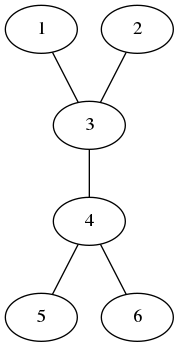
\includegraphics[scale=0.7]{min_graph_4.png}
    \caption{Минимальный граф с критическим ребром между 3-й и 4-й вершинами.}
    \label{fig:min_graph_4}
\end{figure}

Из каждой вершины исходного графа запустим алгоритм Дейкстры.
На каждом шаге работы алгоритма изменяем вес текущего ребра $W(e_i) \rightarrow \gamma W(e_i)$
Затем для данной итерации пересчитаем сумму сетевых расстояний, и, если она меньше текущей минимальной суммы,
то обновим минимум. Так в процессе работы алгоритма мы переберем все ребра и в качестве критического выберем 
ребро с соответствующей минимальной суммой сетевых расстояний. 

\paragraph{}

На каждой итерации работы алгоритма Дейкстры получим сумму сетевых расстояний для исходного графа:
Соответственно для каждой веришны имеем следующую сумму сетевых расстояний:

\paragraph{}

Для первой веришны сумма сетевых расстояний будет состоять из сумм представленных ниже 
путей от первой вершины графа к остальным.
Далее через тире обозначенны вершины графа и сумма весов всех ребер в данном пути:
\begin{gather}
1 - 3 : weight sum = 1 \\
1 - 3 - 4 : weight sum = 5 \\
1 - 3 - 4 - 5 : weight sum = 6 \\
1 - 3 - 4 - 6 : weight sum = 6 \\
1 - 2 : weight sum = 2
\end{gather}
$Sum_1 = 1 + 5 + 6 + 6 + 2 = 20$

\paragraph{}

Для второй веришны сумма сетевых расстояний будет состоять из сумм представленных ниже 
путей от второй вершины графа к остальным.
Далее через тире обозначенны вершины графа и сумма весов всех ребер в данном пути:
\begin{gather}
2 - 3 : weight sum = 1 \\
2 - 3 - 4 : weight sum = 5 \\
2 - 3 - 4 - 5 : weight sum = 6 \\
2 - 3 - 4 - 6 : weight sum = 6 \\
2 - 1 : weight sum = 2
\end{gather}
$Sum_2 = 1 + 5 + 6 + 6 + 2 = 20$

\paragraph{}

Для третьей веришны сумма сетевых расстояний будет состоять из сумм представленных ниже 
путей от третьей вершины графа к остальным.
Далее через тире обозначенны вершины графа и сумма весов всех ребер в данном пути:
\begin{gather}
3 - 1 : weight sum = 1 \\
3 - 2 : weight sum = 1 \\
3 - 4 : weight sum = 4 \\
3 - 4 - 5 : weight sum = 5 \\
3 - 4 - 6 : weight sum = 5 \\
\end{gather}
$Sum_3 = 1 + 1 + 4 + 5 + 5 = 16$

\paragraph{}

Для четвертой веришны сумма сетевых расстояний будет состоять из сумм представленных ниже 
путей от четвертой вершины графа к остальным.
Далее через тире обозначенны вершины графа и сумма весов всех ребер в данном пути:
\begin{gather}
4 - 5 : weight sum = 1 \\
4 - 6 : weight sum = 1 \\
4 - 3 : weight sum = 4 \\
4 - 3 - 1 : weight sum = 5 \\
4 - 3 - 2 : weight sum = 5 \\
\end{gather}
$Sum_4 = 1 + 1 + 4 + 5 + 5 = 16$

\paragraph{}

Для пятой веришны сумма сетевых расстояний будет состоять из сумм представленных ниже 
путей от пятой вершины графа к остальным.
Далее через тире обозначенны вершины графа и сумма весов всех ребер в данном пути:
\begin{gather}
5 - 3 : weight sum = 1 \\
5 - 4 - 3 : weight sum = 5 \\
5 - 4 - 3 - 1 : weight sum = 6 \\
5 - 4 - 3 - 2 : weight sum = 6 \\
5 - 6 : weight sum = 2
\end{gather}
$Sum_5 = 1 + 5 + 6 + 6 + 2 = 20$

\paragraph{}

Для шестой веришны сумма сетевых расстояний будет состоять из сумм представленных ниже 
путей от шестой вершины графа к остальным.
Далее через тире обозначенны вершины графа и сумма весов всех ребер в данном пути:
\begin{gather}
5 - 3 : weight sum = 1 \\
5 - 4 - 3 : weight sum = 5 \\
5 - 4 - 3 - 1 : weight sum = 6 \\
5 - 4 - 3 - 2 : weight sum = 6 \\
5 - 6 : weight sum = 2
\end{gather}
$Sum_6 = 1 + 5 + 6 + 6 + 2 = 20$

\paragraph{}

Таким образом получим сумму сетевых расстояний в исхожном графе $S = 20 + 20 + 16 + 16 + 20 + 20 = 112$.

\begin{figure}[h]
    \centering
    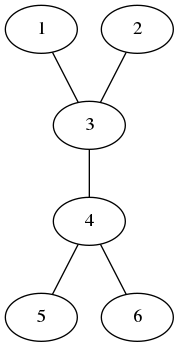
\includegraphics[scale=0.7]{min_graph_2.png}
    \caption{Если уменьшить вес ребра между 3-й и 4-й вершинами сумма сетевых расстояний минимизируется}
    \label{fig:min_graph_2}
\end{figure}

В данном граффе критическим является ребро между
3й и 4й вершинами и умножение его веса на
$\gamma < 1$ приводит к минимизации суммы сетевых расстояний.
При $\gamma = 0.5$ алгоритм меняет вес критического ребра на $0.5 \cdot w_i$ (рис.~\ref{fig:min_graph_2}).

\paragraph{}

На каждой итерации работы алгоритма Дейкстры получим сумму сетевых расстояний для обновленного графа:
Соответственно для каждой веришны имеем следующую сумму сетевых расстояний:

\paragraph{}

Для первой веришны сумма сетевых расстояний будет состоять из сумм представленных ниже 
путей от первой вершины графа к остальным.
Далее через тире обозначенны вершины графа и сумма весов всех ребер в данном пути:
\begin{gather}
1 - 3 : weight sum = 1 \\
1 - 3 - 4 : weight sum = 3 \\
1 - 3 - 4 - 5 : weight sum = 4 \\
1 - 3 - 4 - 6 : weight sum = 4 \\
1 - 2 : weight sum = 2
\end{gather}
$Sum_1 = 1 + 3 + 4 + 4 + 2 = 14$

\paragraph{}

Для второй веришны сумма сетевых расстояний будет состоять из сумм представленных ниже 
путей от второй вершины графа к остальным.
Далее через тире обозначенны вершины графа и сумма весов всех ребер в данном пути:
\begin{gather}
2 - 3 : weight sum = 1 \\
2 - 3 - 4 : weight sum = 3 \\
2 - 3 - 4 - 5 : weight sum = 4 \\
2 - 3 - 4 - 6 : weight sum = 4 \\
2 - 1 : weight sum = 2
\end{gather}
$Sum_2 = 1 + 3 + 4 + 4 + 2 = 14$

\paragraph{}

Для третьей веришны сумма сетевых расстояний будет состоять из сумм представленных ниже 
путей от третьей вершины графа к остальным.
Далее через тире обозначенны вершины графа и сумма весов всех ребер в данном пути:
\begin{gather}
3 - 1 : weight sum = 1 \\
3 - 2 : weight sum = 1 \\
3 - 4 : weight sum = 2 \\
3 - 4 - 5 : weight sum = 3 \\
3 - 4 - 6 : weight sum = 3 \\
\end{gather}
$Sum_3 = 1 + 1 + 2 + 3 + 3 = 10$

\paragraph{}

Для четвертой веришны сумма сетевых расстояний будет состоять из сумм представленных ниже 
путей от четвертой вершины графа к остальным.
Далее через тире обозначенны вершины графа и сумма весов всех ребер в данном пути:
\begin{gather}
4 - 5 : weight sum = 1 \\
4 - 6 : weight sum = 1 \\
4 - 3 : weight sum = 3 \\
4 - 3 - 1 : weight sum = 4 \\
4 - 3 - 2 : weight sum = 4 \\
\end{gather}
$Sum_4 = 1 + 1 + 2 + 3 + 3 = 10$

\paragraph{}

Для пятой веришны сумма сетевых расстояний будет состоять из сумм представленных ниже 
путей от пятой вершины графа к остальным.
Далее через тире обозначенны вершины графа и сумма весов всех ребер в данном пути:
\begin{gather}
5 - 3 : weight sum = 1 \\
5 - 4 - 3 : weight sum = 3 \\
5 - 4 - 3 - 1 : weight sum = 4 \\
5 - 4 - 3 - 2 : weight sum = 4 \\
5 - 6 : weight sum = 2
\end{gather}
$Sum_5 = 1 + 3 + 4 + 4 + 2 = 14$

\paragraph{}

Для шестой веришны сумма сетевых расстояний будет состоять из сумм представленных ниже 
путей от шестой вершины графа к остальным.
Далее через тире обозначенны вершины графа и сумма весов всех ребер в данном пути:
\begin{gather}
5 - 3 : weight sum = 1 \\
5 - 4 - 3 : weight sum = 3 \\
5 - 4 - 3 - 1 : weight sum = 4 \\
5 - 4 - 3 - 2 : weight sum = 4 \\
5 - 6 : weight sum = 2
\end{gather}
$Sum_6 = 1 + 3 + 4 + 4 + 2 = 14$

\paragraph{}

Для обновленного графа, в котором мы заменили вес критического ребра на 2 получим сумму сетевых расстояний:
В таком случае сумма сетевых расстояний для обновленного графа будет равнятся $S^* = 14 + 14 + 10 + 10 + 14 + 14 = 76$.

\paragraph{При $\gamma = 2 > 1$.}
Алгоритм меняет вес критического ребра на $2 \cdot w_i = 8$ (рис.~\ref{fig:min_graph_8}).

\begin{figure}[h]
    \centering
    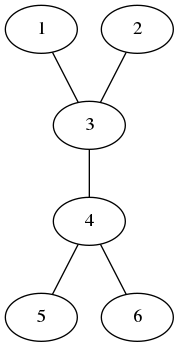
\includegraphics[scale=0.7]{min_graph_8.png}
    \caption{Если увеличить вес ребра между 3-й и 4-й вершинами сумма сетевых расстояний максимизируется}
    \label{fig:min_graph_8}
\end{figure}

В обновленном графе, с весом критического ребра = 8 мы получим следующую
сумму сетевых расстояний:

Что дает сумму сетевых расстояний равную $S^* = 184$

\subsection{Граф малого размера (20 вершин)}

\paragraph{}
При запуске на графе малого размера (рис~\ref{fig:small}) 
алгоритм корректно определил критическое ребро.
Этому ребру был намеренно предан большой вес для удобства тестирования.
При $\gamma = 0.5$ и при $\gamma = 1.5$ алгоритм определял одно
и то же ребро между 19-й и 20-й вершинами (отмечено красным),
однако изменение веса этого ребра приводило к разным итоговым
суммам сетевых расстояний, а именно к $12542$ и $14264$ соотвественно.

\begin{figure}[h]
    \centering
    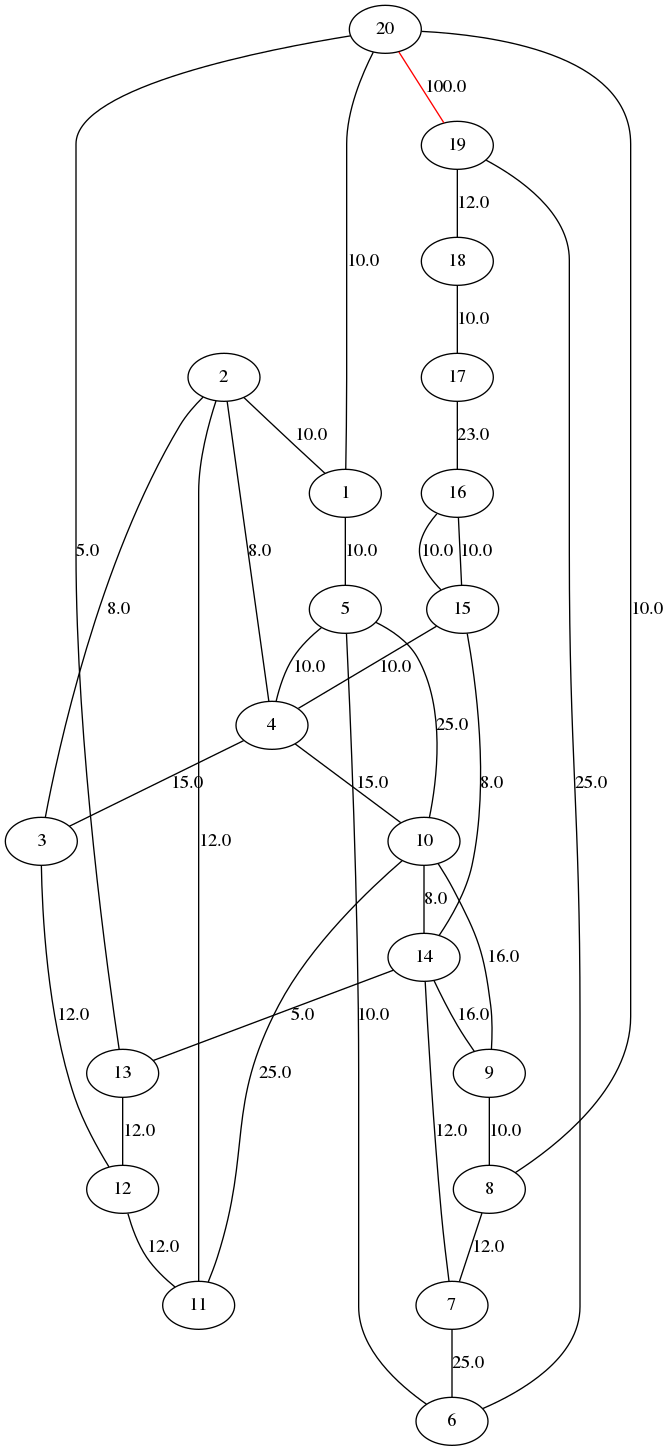
\includegraphics[scale=0.3]{small.png}
    \caption{Малый граф с 20-ю вершинами. Критическое ребро отмечено красным.}
    \label{fig:small}
\end{figure}

\subsection{Граф среднего размера (~1500 вершин)}

\paragraph{}
В качестве графа среднего размера был взят сокращеное представление 
транспортной сети города Владивостока на 2009-й год (рис.~\ref{fig:vlad_2009}). 
В данном представлении 1542 вершины и 1653 ребра.

\begin{figure}[h]
    \centering
    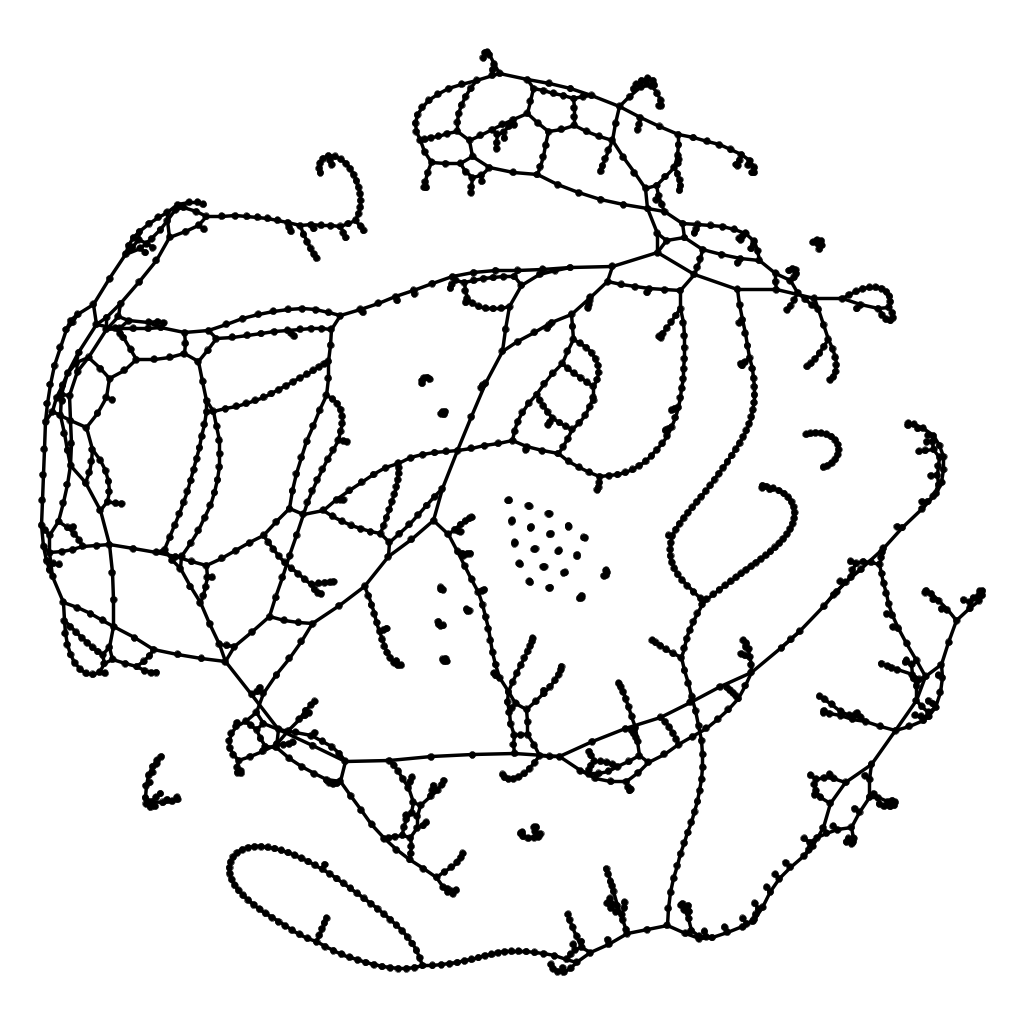
\includegraphics[scale=0.3]{vlad_2009.png}
    \caption{Сокращенная транспортная сеть города Владивостока на 2009-й год.}
    \label{fig:vlad_2009}
\end{figure}

\paragraph{}
Алгоритм был запущен с значениями $\gamma = 0.5$ и $\gamma = 24.5$ и определил 
критическое ребра между 175й и 176й вершиной и между 159-й и 160-й вершинами соответвенно.
На рис~\ref{fig:vlad_2009_min} изображен граф с отмеченными найденными критическими ребрами.
Исходная сумма сетевых расстояний составляет $2.64371\cdot10^{10}$.
При $\gamma = 0.5$ сумма сетевых расстояний составила $2.60341\cdot10^{10}$. 
При $\gamma = 24.5$ сумма сетевых расстояний составила $3.84203\cdot10^{10}$.

\paragraph{}

Без флагов оптимизации нашей программе потребовалось 7 минут 39 секнуд реального времени.
С флагом оптимизации -O2 нашей программе потребовалось 45 секунд реального времени.
Программа использовала 16 потоков. Время измерялось утилитой time.

\begin{figure}[h]
    \centering
    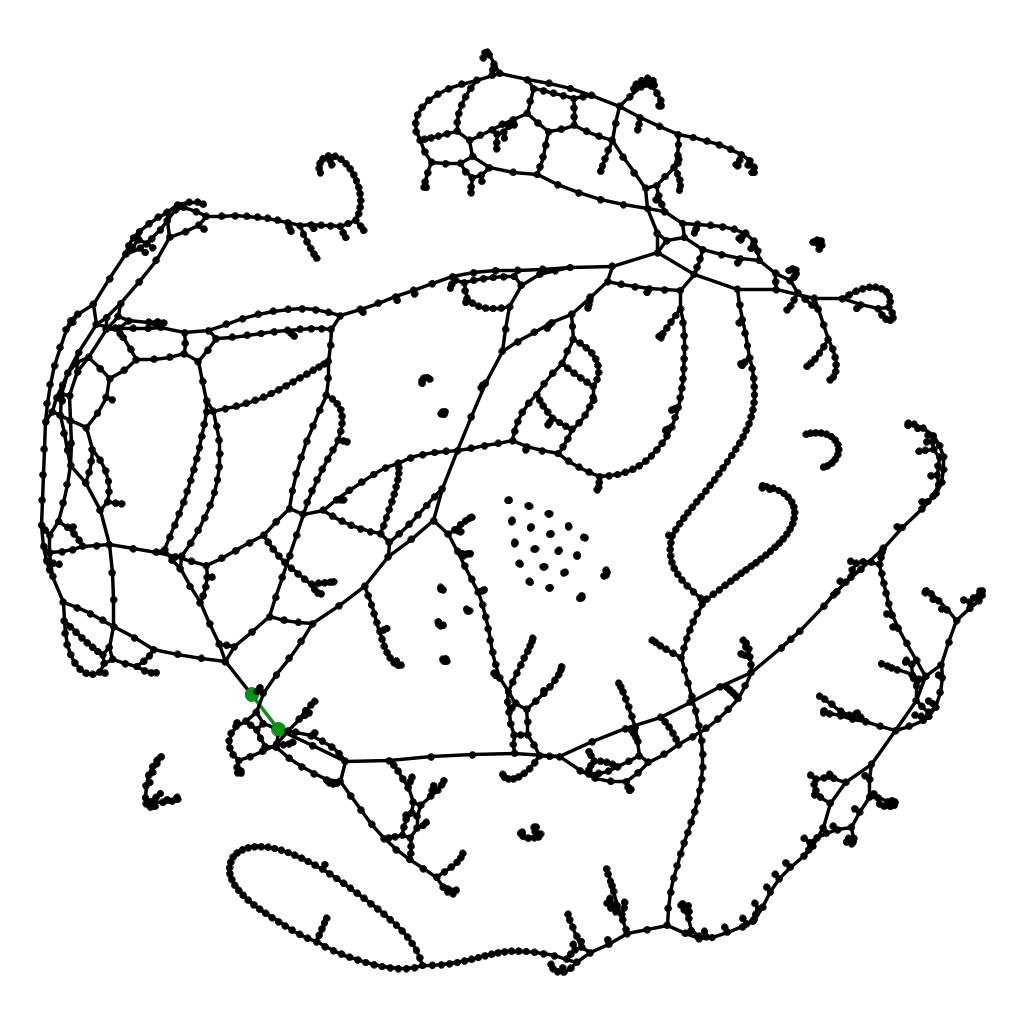
\includegraphics[scale=0.3]{vlad_2009_min.png}
    \caption{Сокращенная транспортная сеть города Владивостока на 2009-й год.}
    \label{fig:vlad_2009_min}
\end{figure}

\section {Инсталляция и запуск}

\paragraph{Генерация отчета}
Файл отчета в формате pdf генерируется также при помощи nuweb. В папке с report.w необходимо выполнить:
$$nuweb\ report.w$$
В результате сгенерируется файл Tex $report.tex$, затем выполнить:
$$pdftlatex\ report.tex$$
Иногда nuweb сам выводит сообщение о том, что требуется сгенерировать tex файл еще раз. Тогда требуется повторить описанные здесь операции.

\paragraph{Запуск программы}

Запуск проводится на orta.dvfu.ru.
Для запуска программы требуется сгенерировать исходные файлы с помощью 
$$nuweb\ report.w$$
Далее перейти в папку src/ и выполнить:

$$cmake\ .$$
$$make$$

Пример запуска:
$$./main\ ../graphs/vlad-2009.dat$$

\section{Заключение}

\paragraph{}
В результате проделанной работы был разработан алгоритм поиска критического ребра в графе.
Алгоритм был протестирован на графах различных размерностей и корректно решил поставленную задачу.

\newpage

\begin{thebibliography}{9}
\bibitem{dijkstra}
Dijkstra E. W. \textit{A note on two problems in connection with graphs} //
\textit{Numer. Math} — Springer Science+Business Media, 1959.
— Vol. 1, Iss. 1. — P. 269–271.
\end{thebibliography}

Для визуализации графов использовалась программа с открытым исходным кодом $gephi$.
https://github.com/gephi/gephi

\end{document}
